\documentclass{article}
\usepackage[utf8]{inputenc}
\usepackage{graphicx}
\usepackage{hyperref}

\title{\textbf{Analyzing the Coffee Landscape: \\\textit{New York City (NYC)}}}
\author{Author: Visaj Nirav Shah}
\date{\emph{September 2020}}

\begin{document}

\maketitle

\section{Problem Statement}
{Analyze neighborhood clusters of \textit{New York City (NYC), USA} based on the number of coffeehouses and cafes present, the ratings, pricing and number of likes of the stores.}
\subsection{Purpose}
{\textit{NYC} is the financial capital \textit{United States of America (USA)}, a popular tourist destination, has a huge population, and houses offices of important international institutions and major corporate headquarters. In such a landscape, coffeehouses are a crucial part of everyday life. People socialize in coffee shops, hold informal group meetings, relax after a long day, and so on. Hence, it is imperative to analyze the coffee scene in such a city where millions depend on a cup of fresh brew.}
\subsection{Target Audience}
{The results of this study will be of particular interest to the major stakeholders mentioned below:-}
\begin{itemize}
    \item \textbf{Major Coffeehouse and Cafe Chains}\\{Corporate chains working in this field can use the results to predict the market opportunities and future growth for their firm. This study will help them select the most profitable next new location.}
    \item \textbf{Prospective Franchisees and Coffeehouse Owners}\\{People wanting to buy franchise stores of chains, like \textit{Starbucks}, \textit{Tim Hortons}, and so on, can understand the landscape and spread of quality stores. This will help them enter the market in a profitable manner with an idea of the competition and target customers.}
    \pagebreak
    \item \textbf{Offices and Public Places}\\{Corporate offices, especially small and medium businesses, need to ensure that their business location is attractive enough to be inviting to customers. Employees and visitors should know the options of going outside for informal meetings, relaxing, and so on.}
    \item \textbf{Tourists and Residents}\\{Tourism is a substantial part of the economy the city. There is a constant and large influx of tourists who visit this city. This project can help the tourists make an informed choice about deciding where to enjoy a cup of refreshing coffee. Similarly, people new to the city or neighborhood can understand the surrounding coffee scene better.}
\end{itemize}
\section{Data}
\textbf{\textit{Places API} - \textit{Foursquare Developers}}\\{\textit{Foursquare Labs Inc.} is a technology product company based in \textit{New York City, USA}. Their primary product is a local search-and-discovery platform. Users can record their check-ins, review everyday places, and add other useful details, experiences, and so on about places they visit.}\\\\{Foursquare collects the information provided by users, and enables developers access the same for development purposes. The information can be retrieved using \textit{Foursquare Developers' Places API}\footnote{Foursquare Developers' Places API:- \url{https://developer.foursquare.com/docs/places-api/}}.}\\\\{The available data is reach with many features. Primarily, for our problem statement, we will use the count of coffeehouses and cafes in a neighborhood and the ratings of locations. For example, number of coffee shops in \textit{Upper East Side, NYC} and the ratings of these locations.}\\\\\\
\textbf{\textit{2014 New York City Neighborhood Names}}\\
{This \textit{New York City Neighborhood Names} point file was created as a guide to \textit{New York City}’s neighborhoods that appear on the web resource, \textit{“New York: A City of Neighborhoods.”} Best estimates of label centroids were established at a 1:1,000 scale, but are ideally viewed at a 1:50,000 scale.\footnote{2014 New York City Neighborhood Names:- \url{https://geo.nyu.edu/catalog/nyu\_2451\_34572}} From this dataset, we are going to get the list of each neighborhood in \textit{NYC}.}\\\\
{This dataset, published by \textit{Department of City Planning, New York (City)} in 2014, is held by \textit{New York University (NYU)} and is available on \textit{NYU Spatial Data Repository}.}
\section{Methodology}
\subsection{Getting the Neighborhoods of \textit{New York City}}\\
{After downloading the dataset from the source mentioned before, the obtained JSON response is converted into a \texit{Pandas} DataFrame named NYNghbor. This is to help us simplify the process of analyzing the data. Using various \texit{Pandas} and \texit{NumPy} functions, we can easily access data and work on it.}\\\\
{NYNghbor contains the Latitude, Longitude and Borough details of the neighborhoods.}\\\\
\begin{figure}[h]
\caption{NYNghbor}
\centering
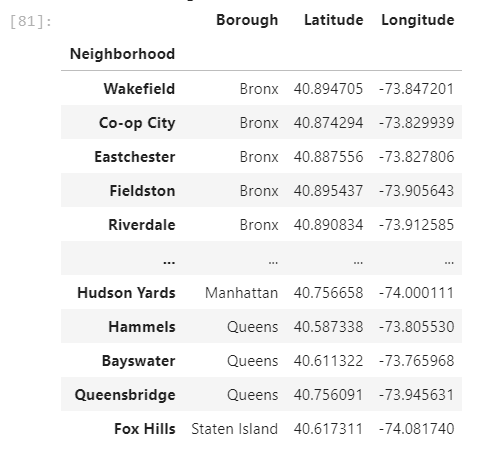
\includegraphics[width=0.5\textwidth]{images/Screenshot (36).png}
\end{figure}\\\\
{Next, we visualize these neighborhoods on a map to get an idea about their location.}\\\\\pagebreak
\begin{figure}[h]
\caption{Neighborhoods Visualized on \textit{NYC} Map}
\centering
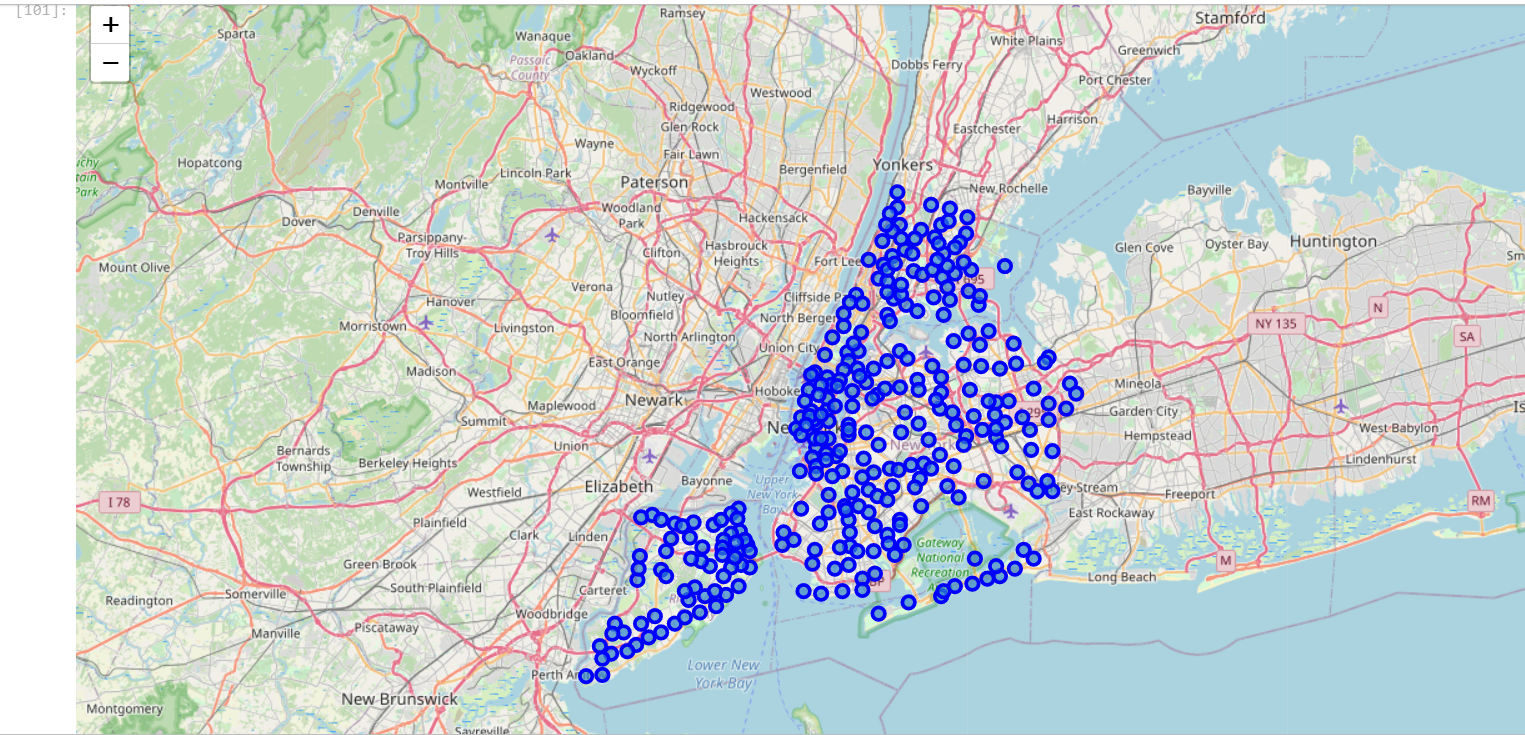
\includegraphics[width=\textwidth]{images/Screenshot (37).png}
\end{figure}\\\\
\subsection{Getting Venues Information}
{We now use the \textit{Foursquare API} to get details of various places in these neighborhoods. We will make a call to this API and then store the JSON response in a DataFrame NYVenues.}\\\\
\begin{figure}[h]
\caption{NYVenues.head()}
\centering
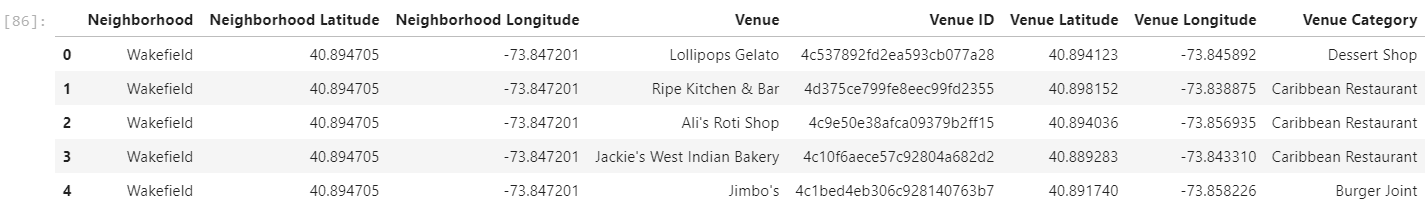
\includegraphics[width=\textwidth]{images/Screenshot (38).png}
\end{figure}\\\\
\subsubsection{Filtering out Coffee shops and Cafes}
{From the various locations obtained, we need to filter out the Coffee shops and Cafes, which are of interest for our problem. This filtering is carried out by using the two commands given below:-}\\
\begin{center}
    {NYVenues.loc[NYVenues['Venue Category'].str.contains('Coffee')]}\\{NYVenues.loc[NYVenues['Venue Category'] == 'Café']}
\end{center}
{Now we make API calls to \textit{Foursquare API} for getting individual details like ratings, price tier, likes, etc. of each coffee location. All these details will be stored in a DataFrame coffee.}
\begin{figure}[h]
\caption{coffee.head()}
\centering
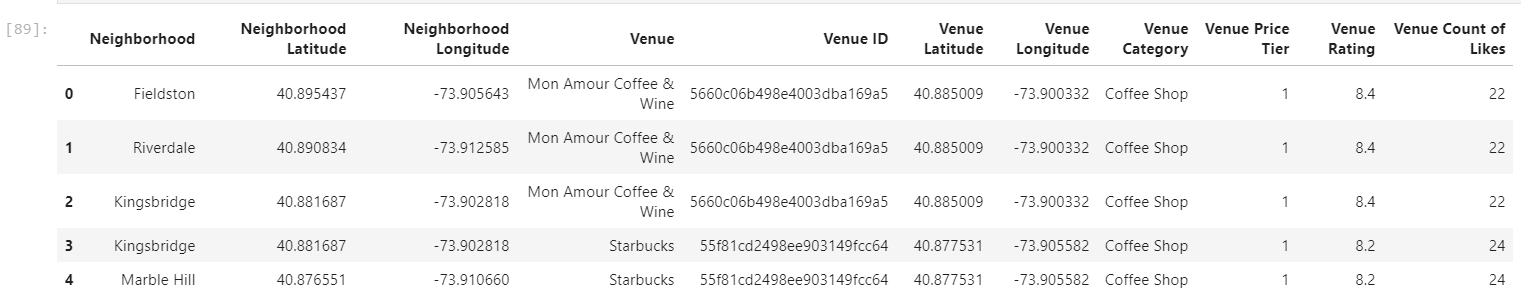
\includegraphics[width=\textwidth]{images/Screenshot (39).png}
\end{figure}
\subsection{Clustering the Neighborhoods}
{Before we begin clustering the neighborhoods, let's take a brief overview of the data grouped by the neighborhoods.}
\subsubsection{Grouped by Neighborhoods Data}
{We observe that there are 214 neighborhoods in coffee. We will be clustering these 214 neighborhoods.To get details for each neighborhood, we create a DataFrame NYNghborCoffee}\\\\
{NYNghborCoffee will store the Number of locations in the neighborhood, Average Price Tier, Average Ratings and Average number of Likes of locations in the neighborhood.}
\begin{figure}[h]
\caption{NYNghborCoffee.head()}
\centering
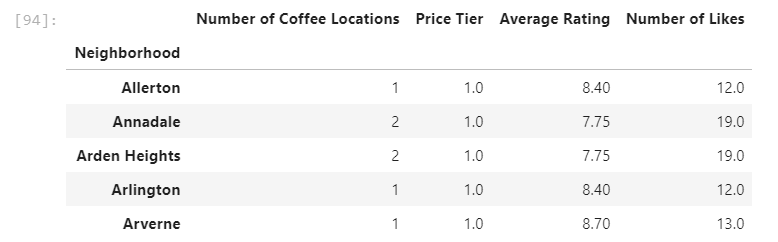
\includegraphics[width=\textwidth]{images/Screenshot (40).png}
\end{figure}
\\\\
{Now, we begin the Clustering Procedure.}
\\\\\\\\\\
{For clustering, we will use the k-means algorithm. We will implement the algorithm using \textit{scikit-learn} library available for \textit{Python}.}\\\\
{To determine the perfect k (i.e. the number of clusters), we loop through a reasonable range of k values. Here, this range is [2, 10].}\\\\
{For each k, we plot the SSE (i.e. Sum of Squared Distance) and then using the Elbow Method, we determine the required k.}\\\\
{According to the Elbow Method, the best k is the one after which the SSE vs. k plot is almost linear and has very little change in slope.}\\\\
{For better results, we will standardize the data before calculating the SSE. This means the mean of each column will be 0 and the standard deviation will be 1.}
\begin{figure}[h]
\caption{Plot for Elbow Method}
\centering
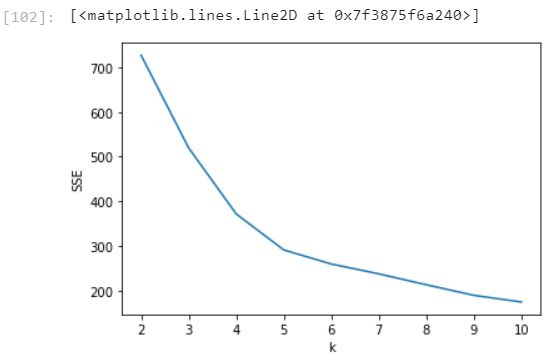
\includegraphics[width=\textwidth]{images/Screenshot (42).png}
\end{figure}\\\\
{After looking at this plot, we can clearly say that k = 5 is a reasonable choice for number of clusters. We run the k-means algorithm for our data keeping k = 5.}
\pagebreak
\section{Results}
{After running the algorithm, we get an array, shown below, with cluster number for each neighborhood.}
\begin{figure}[h]
\caption{Output of k-means clustering}
\centering
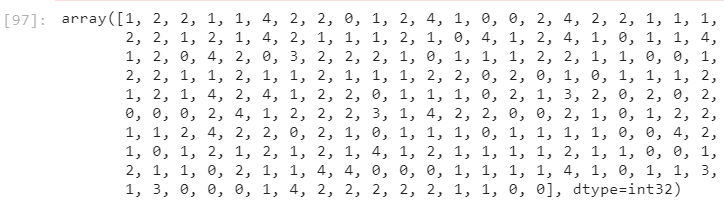
\includegraphics[width=\textwidth]{images/Screenshot (45).png}
\end{figure}\\\\
{We will add this as a column to our NYNghborCoffee DataFrame so that all the information is consolidated in one place.}
\begin{figure}[h]
\caption{NYNghborCoffee.head() after adding Cluster Number}
\centering
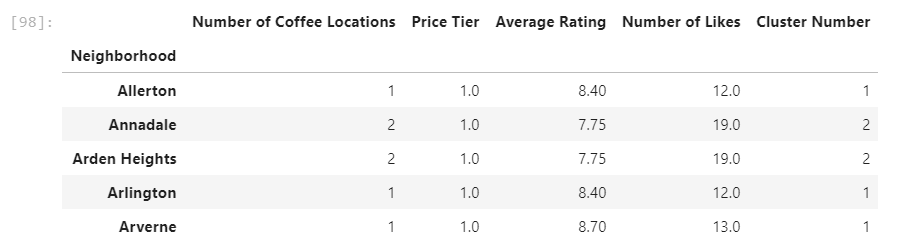
\includegraphics[width=\textwidth]{images/Screenshot (43).png}
\end{figure}\\\\
{To understand the results cluster-wise, we will group NYNghborCoffee by Cluster Number and analyze the results.}
\begin{figure}[h]
\caption{Description of Each Cluster}
\centering
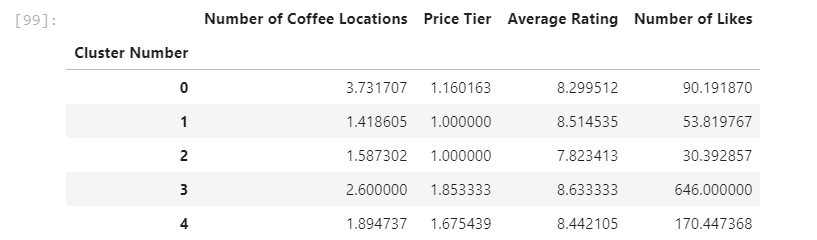
\includegraphics[width=\textwidth]{images/Screenshot (44).png}
\end{figure}\\
{Further analysis in the Discussion section.}
\section{Discussion}
{Based on the cluster descriptions obtained, we can make the following observations and recommendations:-}
\begin{itemize}
    \item \textbf{Cluster 3} has the best coffee places in the city. With highest number of likes and highest average rating, these locations are extremely popular. The stores in this cluster are a bit pricey, but they serve products worth the price given the popularity and demand. Difficult for new stores to make a mark since there is little scope of improving customer experience.
    \item \textbf{Cluster 4} is again a coffee-friendly cluster but with reduced number of locations. The density of stores is less, but customers have vouched for the quality of service (high ratings and number of likes). This cluster is a good choice for newcomers in the business who plan to start a non-franchise store. Given the demand but less number of locations, newcomers stand a good chance of attracting customers.
    \item \textbf{Cluster 0} is not a good place for new businesses. The density of stores is very high as compared to others and popularity is low. The ratings and number of likes are lower than Cluster 3 and 4. Possible reasons for low popularity could include unsatisfactory service and products, or inherent nature of locations such that the demand for coffee is less. In either case, rather than new stores opening, some of the old ones may be pulling down the shutters forever. One possibility for high number of stores and low demand could mean that there are a lot of corporate coffee shops meaning the ones managed by companies exclusively for their employees and clients. 
    \item \textbf{Cluster 1} has a low density of stores but positive ratings. Given the low number of likes, one can deduce that not many are coffee-consumers, but those who do, have good options available. One could consider opening a store here since there is a demand (specific audience) but the number of options are really less. So, there is a high probability that people are willing to test new options and possibly make a shift. If you come up with some unique feature for your store, it could generate interest among both, regular customers, and new customers.
    \item \textbf{Cluster 2} is clearly not a good place to open a coffee shop, or the best if you are a risk-taker and want to risk entering a completely new domain. These neighborhoods have very few stores, but since there are few people to drink, there are not many changes taking place in the landscape. Given the low ratings, people are probably not happy with their current options, so new stores could stand a chance of attracting the crowd, but they need to be really good to get people to drink coffee.
\end{itemize}
\pagebreak
\section{Conclusion}
{All in all, after looking at the results and analyzing the process, one can decide on a location depending on their requirements. After understanding the Coffee landscape, people are now equipped to make intelligent business decisions and churn out maximum profits depending on the objectives. Also, as explained at the beginning, this study can empower tourists and citizens too, not only businesses.}
\subsection{Possible Improvements and Future Scope}
{Clearly, this is not an exhaustive model for analysis. Some other factors which can be included are area of each neighborhood, population of individual neighborhood, real estate prices, on-field public response, and so on.}\\\\
{This study could be expanded to other major cities across the world as well. This should be of help, especially to multi-national companies. Detailed analysis for entire countries can help them understand the soft spots of their business model and market.}
\end{document}
